\documentclass[a4paper,12pt]{scrreprt}
\usepackage[utf8]{inputenc}

\usepackage[ngerman]{babel}
\usepackage[x11names]{xcolor}
%\renewcommand{\familydefault}{\sfdefault}

\usepackage{ifpdf}
\ifpdf
\usepackage[pdftex]{graphicx}
\else
\usepackage{graphicx}
\fi

% Title Page

\title{Hardware Modellierung LU}
\author{Nick Mayerhofer, Lukas Petermann}

\begin{titlepage}
    \vspace*{\stretch{1}}
    \HRule
    \begin{center}
        \LARGE Spezifikation \\
        Taschenrechner
    \end{center}
    \HRule
    \vspace*{\stretch{2}}
    \begin{center}
        \Large Hardware Modeling SS 2010 \\
        
     \end{center}
    \vspace*{\stretch{3}}
    \begin{center}
        \large Gruppe 11 \\
        \vspace{30pt}
        \normalsize Nick Mayerhofer \\
        0726179 \\
        \vspace{15pt}
        Lukas Petermann \\
        0725146
     \end{center}
     \vspace*{\stretch{4}}
 \end{titlepage}

\begin{document}
%\maketitle
\tableofcontents

%macht korrekte Nummerierung
\renewcommand{\thesection}{\arabic{section}}

\chapter{Hardware Modellierung LU}

\section{Einleitung}

Dieses Dokument beschreibt die Spezifikationen eines einfachen Rechners der die vier Grundrechnungsarten unterstützt.
Welcher im Zuge der LU Hardware Modellierung zu realisieren ist.\\
Eingaben werden über die Tastatur gemacht. Erlaubt sind die Zahlen '0'-'9', die vier Operationszeichen auf dem Ziffernblock, 
die Leer-, Backspace- und Entertaste des normalen Blocks.\\
Die Ausgabe erfolgt über den VGA Port des development Boards und somit auf einen Monitor. Jede Rechnung darf bis zu 70 Zeichen lang sein und das Ergebnis wird nach drücken der Entertaste
in der nächsten Zeile ausgegeben. Sollte man sich bereits in der letzten Zeile befinden, werden die restlichen Zeilen um eine Zeile nach oben
verschoben.\\
Der Taschenrechner speichert die letzten 50 Rechnungen und kann diese auf Anfrage über das RS232 Interface verschicken.

Implementiert ist auch eine Fehlerbehandlung um keine falschen Ergebnisse zu liefern. Abgedeckt ist die Division durch Null, Overflows von
Zahlen- und Ergebnissen sowie die ungültige Positionierung von Operanden.


\section{Requirements}
%%%%%%%%%%%%%%%%%%%%%%%%%%%%%%TODO Schreiben
kommt da her



\begin{enumerate}
 \item TC1 : Addition zweier Zahlen
 \item TC2 : Subtraktion zweier Zahlen
 \item TC3 : Multiplikation zweier Zahlen
 \item TC4 : Division zweier Zahlen
 \item TC5 : Verkettung aller Grundrechnungsarten
 \item TC6 : Punkt vor Strichrechnung
 \item TC7 : zu große Zahlen verwenden
 \item TC8 : Division durch 0
 \item TC9 : zwei Operatoren hintereinander, 
 \item TC10 : Operator am Ende
 \item TC11 : Überlange Eingabe
 \item TC12 : Leertase erzeugt einen Abstand der bei der Berechnung ignoriert wird.
 \item TC13 : Backspace l�scht uns das letzte Zeichen
 \item TC14 : Auslesen der History
 \item TC15 : Fehlermeldung f�r Division durch Null
 \item TC16 : Fehlermeldung f�r einen Syntax Fehler
 \item TC17 : Fehlermeldung f�r einen Overflow
 \item TC18 : Divisionen werden abgerundet

\end{enumerate}



\section{High level design description}

Der Rechner wurde so entworfen, dass sich die einzelnen Teilaufgaben möglichst einfach in eigene Module
kapseln lassen. Dies erleichtert die Implementierung, Wartung und spätere Erweiterung des Gesamtsystems.
Wie diese miteinander kommunizieren wird in folgender Abbildung gezeigt.

\begin{center}
\begin{figure}[!ht]
 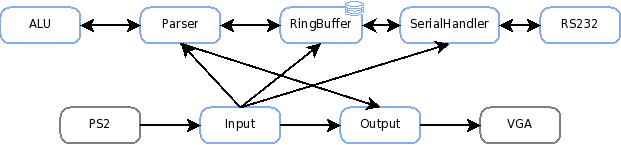
\includegraphics[scale=0.55]{pics/Modules.png}
 % Modules.png: 501x145 pixel, 72dpi, 17.67x5.12 cm, bb=0 0 501 145
 \label{fig:Modules}
\end{figure}
\end{center}

%%%%%%%%TODO Beschreibung der Submodule
\begin{description}
 \item[Input:] Wartet auf Scancodes vom PS2 Modul, bearbeitet diese und schickt, je nach Scancodes, 
ein ASCII Zeichen oder einen Befehle an eine andere Komponente weiter.
 \item[Output:] Bei jedem neuen Zeichen oder nach dem Lösen einer Rechnung muss der Bildschirm aktualisiert werden.
Der Output ist die Schnittstelle zwischen den anzuzeigenden Zeichen und der VGA Komponente, die den Bildschirm 
aktualisiert.
 \item[Parser:] Der Parser wartet auf ein Signal, welches durch das Drücken der Enter Taste ausgelöst wird. Danach holt er sich vom
Ringbuffer Modul die letzte Rechnung, zerlegt diese in seine Grundrechnungen und schickt jede dieser Rechnungen an die ALU.
Nachdem die Berechnung gelöst wurde, wird das Ergebnis an den Ringbuffer und den Output geschickt.
 \item[ALU:] Die ``Arithmetic Logical Unit'' löst die Grundrechnungsarten. Der Parser sendet zwei Operanden und den Operator an die ALU 
und bekommt das Ergebnis zurückgeschickt. 
 \item[Ringbuffer:] Dieses Modul speichert die letzten 50 Rechnungen samt Ergebnissen in einer Ringbuffer Struktur. 
 \item[SerialHandler:] Auf ein Signal vom RS232 oder vom Input Modul holt sich der SerialHandler den gesamten Speicher vom Ringbuffer 
und sendet ihn an die RS232 Komponente.
 \item[RS232:] Dieses Modul hört auf dem RS232 Interface auf den Befehl alle Rechnungen zu schicken und leitet diesen Befehl an den
SerialHandler weiter. Alle Daten die vom SerialHandler kommen werden über das Interface geschickt.
 \end{description}

\subsection{Externe Schnittstellen}
Die folgenden zwei IP-Cores stehen uns zur Lösung der Aufgabe zur Verfügung und müssen nur noch von uns implementiert werden.
\begin{description}
 \item[PS2:] Das PS2 Modul ist die Schnittstelle zwischen der Tastatur und dem Programm. Jeder Tastendruck sendet 1-3 
Scancodes an unser Input Modul und muss daraus den richtige Befehl interpretieren.
 \item[VGA:] Die VGA Komponente erlaubt einfache Kontrolle über den Bildschirm. Mit mehreren Befehlen kann der Bildschirm
verändert werden.
 \end{description}

\subsection{Reset and Clock}
\begin{description}
\item[Der Reset] wurde low active gewählt.

\item[Der VGA] Controller wird über eine PLL auf 25.175 MHz getaktet. 
Alle weiteren Controller benützen die externe Clockfrequenz
des Developer Boards von 33.33 MHz.
 \end{description}


\subsection{Logical Interfaces}
%Die schon gezeigten Module besitzen folgende I/Os:
%\begin{figure}[!ht]
% 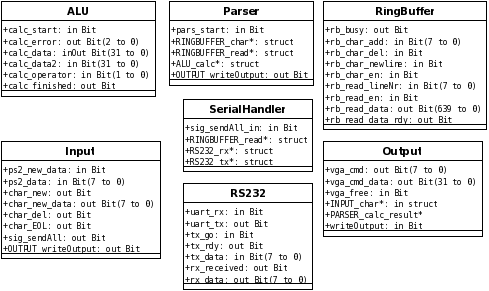
\includegraphics[scale=0.7]{pics/Klassen.png}
 % Modules.png: 501x145 pixel, 72dpi, 17.67x5.12 cm, bb=0 0 501 145
% \label{fig:Klassen}
%\end{figure}

%\subsubsection{Input}

In den folgenden Tabellen 1.1 bis 1.7 findet man die zu den jeweiligen
Komponenten gehörenden Signale inkl. Orientierung und Kurzbeschreibung 
sowie die benötigte Bitbreite.

\begin{table}[h]
 \caption{\textbf{Input Modul}}
 \begin{center}
  \begin{tabular}{|p{4cm}|p{1,6cm}|p{1cm}|p{9cm}|}
   \hline Signal & Richtung & Bits & Beschreibung\\
   \hline
   ps2\_new\_data & in & 1 & Ist High wenn ein neuer Scancode gelesen werden kann.\\
   ps2\_data & in & 8 & Auf diesem Signal liegt der letzte Scancode\\
   inp\_new\_data & out & 1 & Ist High wenn ein neuer gültiger ASCII Code eingegeben wurde.\\
   inp\_data & out & 8 & Der neue gültige ASCII Code.\\
   inp\_del & out & 1 & Beim Drücken der Backspace Taste für einen Zyklus auf High.\\
   inp\_sendRS232 & out & 1 & Wird beim Button auf dem Entwicklerboard ausgelöst.\\
   pars\_start & out & 1 & Beim Drücken der Enter Taste wird der Parser gestartet.\\ 
   \hline
  \end{tabular}
 \end{center}
\end{table}

%\subsubsection{Output}
 
\begin{table}[!h]
 \caption{\textbf{Output Modul}}
 \begin{center}
  \begin{tabular}{|p{4cm}|p{1,6cm}|p{1cm}|p{9cm}|}
   \hline Signal & Richtung & Bits & Beschreibung\\
   \hline
   vga\_command & out & 8 & Befehl an das VGA Modul.\\
   vga\_command\_data & out & 32 & Daten für den Befehl an die VGA.\\
   vga\_free & in & 1 & Signal von der VGA. Erlaubt neue Befehle.\\
   inp\_new\_data & in & 1 & Ist High wenn ein neuer gültiger ASCII Code eingegeben wurde.\\
   inp\_data & in & 8 & Der neue gültige ASCII Code.\\
   inp\_del & in & 1 & Beim Drücken der Backspace Taste für einen Zyklus auf High.\\
   pars\_new\_data & in & 1 & Vom Parser kann ein neuer ASCII Code gelesenw erden.\\
   pars\_data & in & 32 & Der neue ASCII Code.\\
   \hline
  \end{tabular}
 \end{center}
\end{table}

%\subsubsection{Parser}
\begin{table}[!h]
\caption{\textbf{Parser Modul}}
 \begin{center}
  \begin{tabular}{|p{4cm}|p{1,6cm}|p{1cm}|p{9cm}|}
   \hline Signal & Richtung & Bits & Beschreibung\\
   \hline
   ps\_start & in & 1 & Startet Berechnung.\\
   calc\_data & out & 32 & Erster Operand.\\
   calc\_data2 & out & 32 & Zweiter Operand.\\
   calc\_operator & out & 2 & Operator für Berechnung.\\
   calc\_start & out & 1 & Startet Berechnung.\\
   calc\_finished & in & 1 & Berechnung fertig.\\
   calc\_result & in & 32 & Ergebnis.\\
   calc\_status & in & 2 & Status der Berechnung. Bei 0 fehlerfrei, sonst fehlerhaft.\\
   pars\_new\_data & out & 1 & Vom Parser kann ein neuer ASCII Code gelesenw erden.\\
   pars\_data & out & 8 & Der neue ASCII Code.\\
   rb\_busy & in & 1 & Wenn der Buffer beschäftigt ist dürfen keine neuen Eingaben kommen.\\
   rb\_read\_en & out & 1 & Eine neue Zeile wird angefordert.\\
   rb\_read\_lineNr & out & 6 & Die neue Zeile die gelesen werden soll.\\
   rb\_read\_data\_rdy & in & 1 & Die neue Zeile kann gelesen werden.\\
   rb\_read\_data & in & 648 & Die neue Zeile.\\
   \hline
  \end{tabular}
 \end{center}
\end{table}

%\subsubsection{ALU}

\begin{table}[!h]
\caption{\textbf{ALU Modul}}
 \begin{center}
  \begin{tabular}{|p{4cm}|p{1,6cm}|p{1cm}|p{9cm}|}
   \hline Signal & Richtung & Bits & Beschreibung\\
   \hline
   calc\_data & in & 32 & Erster Operand.\\
   calc\_data2 & in & 32 & Zweiter Operand.\\
   calc\_operator & in & 2 & Operator für Berechnung.\\
   calc\_start & in & 1 & Startet Berechnung.\\
   calc\_finished & out & 1 & Berechnung fertig.\\
   calc\_result & out & 32 & Ergebnis.\\
   calc\_status & out & 2 & Status der Berechnung. Bei 0 fehlerfrei, sonst fehlerhaft.\\
   \hline
  \end{tabular}
 \end{center}
\end{table}

%\subsubsection{Ringbuffer}

\begin{table}[!h]
 \caption{\textbf{Ringbuffer Modul}}
 \begin{center}
  \begin{tabular}{|p{4cm}|p{1,6cm}|p{1cm}|p{9cm}|}
   \hline Signal & Richtung & Bits & Beschreibung\\
   \hline
   rb\_busy & out & 1 & Wenn der Buffer beschäftigt ist dürfen keine neuen Eingaben kommen.\\
   pars\_new\_data & in & 1 & Neue Daten von Parser.\\
   pars\_data & in & 8 & Der neue ASCII Code vom Parser.\\
   inp\_new\_data & in & 1 & Neue Daten vom Input\\
   inp\_data & in & 8 & Der neue gültige ASCII Code vom Input.\\
   inp\_del & in & 1 & Ist kurz High wenn ein Zeichen gelöscht werdne soll.\\
   %rb\_char\_add & out & 1 & ??.\\
   %rb\_char\_del & in & 1 & \\
   rb\_char\_newline & in & 1 & Springt in die nächste Zeile.\\
   %rb\_char\_en & in & 1 & \\
   rb\_read\_en & in & 1 & Eine neue Zeile wird angefordert.\\
   rb\_read\_lineNr & in & 6 & Die neue Zeile die gelesen werden soll.\\
   rb\_read\_data\_rdy & out & 1 & Die neue Zeile kann gelesen werden.\\
   rb\_read\_data &out & 648 & Die neue Zeile.\\
   \hline
  \end{tabular}
 \end{center}
\end{table}

%\subsubsection{SerialHandler}

\begin{table}[!h]
\caption{\textbf{SerialHandler Modul}}
 \begin{center}
  \begin{tabular}{|p{4cm}|p{1,6cm}|p{1cm}|p{9cm}|}
   \hline Signal & Richtung & Bits & Beschreibung\\
   \hline
   inp\_sendRS232 & in & 1 & Initialisiert das Senden des gesamten Speichers.\\
   rb\_busy & in & 1 & Wenn der Buffer beschäftigt ist dürfen keine neuen Eingaben kommen.\\
   rb\_read\_en & out & 1 & Eine neue Zeile wird angefordert.\\
   rb\_read\_lineNr & out & 6 & Die neue Zeile die gelesen werden soll.\\
   rb\_read\_data\_rdy & in & 1 & Die neue Zeile kann gelesen werden.\\
   rb\_read\_data & in & 648 & Die neue Zeile.\\
   tx\_rdy & in & 1 & Zum Senden muss rdy low sein.\\
   tx\_go & out & 1 & Startet Sendevorgang.\\
   tx\_data & out & 8 & Das zu sendende Byte.\\
   rx\_recv & in & 1 & Neues Byte wurde empfangen.\\
   rx\_data & in & 8 & Das neue Byte.\\
   \hline
  \end{tabular}
 \end{center} 
\end{table}


%\subsubsection{RS232}

\begin{table}[!h]
 \caption{\textbf{RS232 Modul}}
 \begin{center}
  \begin{tabular}{|p{4cm}|p{1,6cm}|p{1cm}|p{9cm}|}
   \hline Signal & Richtung & Bits & Beschreibung\\
   \hline
   uart\_rx & in & 1 & Die Receive Leitung des UART.\\
   uart\_tx & out & 1 & Die Transmit Leitung des UART.\\
   tx\_rdy & out & 1 & Zum Senden muss rdy low sein.\\
   tx\_go & in & 1 & Startet Sendevorgang.\\
   tx\_data & in & 8 & Das zu sendende Byte.\\
   rx\_recv & out & 1 & Neues Byte wurde empfangen.\\
   rx\_data & out & 8 & Das neue Byte.\\
   \hline
  \end{tabular}
 \end{center}
\end{table}

\subsection{Behavioural Interface}
\subsubsection{Ausgabe am Bildschirm}
Der Bildschirm kann 80 Zeichen in einer Zeile darstellen und unsere Rechnungen können 70 Zeichen lang sein. Mit einem '=' 
Zeichen würden uns 9 Zeichen für das Ergebnis bleiben. Unser Ergebnis ist jedoch 32 Bit lang und liegt zwischen [2147483648,-2147483647].\\
Deswegen und auch wegen der Übersicht schreiben wir das Ergebnis in die nächste Zeile.\\
Der Bildschirmhintergrund ist schwarz mit weißer Schrift. Die Rechnung beginnt in der ersten Zeile. Sollten keine Zeilen mehr 
frei sein rutschen alle Rechnungen um eine Zeile nach oben und die älteste Rechnung wird gelöscht.
\subsubsection{Ausgabe über RS232}
Wird der Button am Developer board, oder eine bestimmte Taste am PC, gedrückt, wird der gesamte Verlauf der letzten 50 Rechnungen inkl. der Ergebnissen an den PC geschickt.
\subsubsection{Umgang mit Overflows}
Overflows werden von unserem ALU Modul abgefangen. Tritt ein Overflow auf wird die Berechnung beendet und eine Fehlernachricht in die History gespeichert.
\subsubsection{Erlaubte Eingabe über die Tastatur}
%%%%%%%%%%%%%%%%%%%%%%%%%%%%%%%%%%%%%%%%%%%
%%%Input from detailed design description
%%%%%%%%%%%%%%%%%%%%%%%%%%%%%%%%%%%%%%%%%%%
Das Programm reagiert nur auf gedrückte und nicht auf losgelassene Tasten. Weiters verwenden wir die Scankeys der 
Zahlen und Operatoren vom NumPad und Enter, Leertaste und Backspace von der Haupttastatur.
\begin{center}
\begin{tabular}{|l|l|l|}
\hline ASCII & Scankey (Set2) & ASCII (hex)\\
\hline 0 & 0x70 & 30\\
1 & 0x69 & 31\\
2 & 0x72 & 32\\
3 & 0x7a & 33\\
4 & 0x6b & 34\\
5 & 0x73 & 35\\
6 & 0x74 & 36\\
7 & 0x6c & 37\\
8 & 0x75 & 38\\
9 & 0x7d & 39\\
+ & 0x79 & 2B\\
- & 0x7b & 2D\\
/ & 0xe0 0x4a & 2F\\
$*$ & 0x7c & 2A\\
Backspace & 0x66 & 08\\
Enter & 0x5a & 0A\\
Space & 0x29 & 20\\
\hline

\end{tabular}
\end{center}
\subsubsection{Fehlerhafte Eingaben}
Alle Tastenereignisse von Tasten die nicht spezifiziert sind werden verworfen. Bei fehlerhaften Eingaben wird der Fehler vom Parser und der ALU abgefangen, die Zwischenergebnisse verworfen, die entsprechende Fehlernachricht am Bildschirm ausgegeben und in der History gespeichert.
\subsubsection{Fehlernachrichten}
Wir unterscheiden zwischen drei Fehlernachrichten (siehe auch \ref{sec_requirements}): 
\begin{description}
 \item[Overflow] Wenn bei irgendeiner Berechnung ein Overflow Fehler auftritt. 
 \item[Division durch Null] Sollte bei Irgendeiner Division im Zähler null stehen wird diese Nachricht ausgegeben.
 \item[falscher Syntax]Zu falscher Syntax zählt ein Operand am Ende, zwei Operanden hintereinander oder eine Punktrechnung am Anfang.
\end{description}


\subsection{Physical Interfaces}
Die Physikalischen Interfaces der gesamten angeschlossenen Hardware lässt sich
in nachfolgender Pintabelle ablesen.
\begin{table}[!ht]
 \begin{center}
  \begin{tabular}{|l|l|l|l|}
   \hline Signal & Pin &Direction &Logic Level\\
   \hline
   sys\_clk & N3 & in & LVTTL\\
   sys\_res\_n & AF17 & in & LVTT\\
   btn\_a & A3 & in & LVTTL\\
   uart\_cts & D20 & out & LVTTL\\
   uart\_rts & D21 & in & LVTTL\\
   uart\_txd & D22 & out & LVTTL\\
   uart\_rxd & D23 & in & LVTTL\\
   ps2\_data & E21 & bidirec & LVTTL\\
   ps2\_clk & Y26 & bidirect & LVTTL\\
   vga\_r0 & E22 & out & LVTTL\\
   vga\_r1 & T4 & out & LVTTL\\
   vga\_r2 & T7 & out & LVTTL\\
   vga\_g0 & E23 & out & LVTTL\\
   vga\_g1 & T5 & out & LVTTL\\
   vga\_g2 & T24 & out & LVTTL\\
   vga\_b0 & E24 & out & LVTTL\\
   vga\_b1 & T6 & out & LVTTL\\
   vga\_hsync\_n & F1 & out & LVTTL\\
   vga\_vsync\_n & F2 & out & LVTTL\\
   \hline
  \end{tabular}
 \end{center}
\end{table}

\newpage


\section{Detailed design description}

%%%%%%%%%%%%%%%%%%%%%%%%%%%%%TODO genaue Beschreibung hier rein

% \begin{itemize}
% \item Description how the design will be implemented
% \item Event sequence digrams
% \item Internal structure
% 	\begin{itemize}
% 	\item Memory
% 	\item Logic blocks
% 	\item Parallel processes
% 	\item State machines
% 	\end{itemize}
% \end{itemize}
\subsection{ALU}
Die Alu führt nach dem Startsignal die am \textit{operation}seingang gewählte 
Rechenoperation ausgeführt. Dazu stehen folgende Optionen am operationseingang zur Verfügung:
\begin{center}
% use packages: array
\begin{tabular}[!ht]{|l|l|l|}
\hline Eingang (binär) & Rechenoperation & Rechnungsart\\ 
	00 & Addieren & Strichrechnung\\ 
	01 & Subtrahieren & Strichrechnung\\ 
	10 & Multiplizieren & Punktrechnung\\ 
	11 & Dividieren & Punktrechnung\\
 \hline
\end{tabular}
\end{center}
Die division schneidet nachkommastellen ab.
Die dafür benötigten Fälle werden anhand von cases unterschieden.
\subsection{Parser}
Den Parser arbeitet mit zwei Integer Puffern. \\
Nach starten des Parsers werden sukzessive alle sich in einer Zeile befindenden CHARs durchgearbeitet.

wird die erste Zahl gefiltert und in den \textit{Punktrechnungsbuffer} geschoben.
Folgt eine
\subsection{Ringbuffer}
Ringbuffer Funktionalitäten:
\begin{itemize}
 \item Hinzufügen eines CHARs zu der aktuellen Zeile
 \item Löschen des letzten CHARs der aktuellen Zeile
 \item Wechseln in die nächste Zeile
 \item Auslesen einer gesamten Zeile mit konkreter Nummer
 \item Ressource blockierbarkeit
\end{itemize}
Aktuelle Zeile des Ringbuffers wird immer mit dem Wert 0 gekennzeichnet.

\subsection{RS232}
Das RS232 Modul überwacht die Empfangsleitung und stellt nach Empfang die Daten auf einem 
8 Bit Bus zur Verfügung.\\
Beim Senden bezieht es 8 Bit von dem Eingangsbus und meldet den Versandt über ein ready Bit.

Beide Modi arbeiten mit 8 Datenbits, einem Stopbit und keinem paritätsbit, bei einer
Boudrate von 115`200
%Senden: TX->LOW alle 8.68us nächstes Bit, dann 1 zum Stoppen
\subsection{Input}
Input arbeitet die vom ps/2 Modul empfangenen Daten ab und sendet diese je nach Empfangsdaten weiter.\\
Unterscheidung der Empfangenen Daten:
\begin{description}
 \item[0-9,+,-,*,/] 
	\begin{itemize}
		\item Wandeln der Scancodes in ASCII chars 
		\item Speichern der Chars im RingBuffer
		\item Senden der Chars an den Output
	\end{itemize}
 \item[Enter] Senden an Parser und Output
 \item[Backspace] Senden an RingBuffer und Output
 \item[Space] Senden an RingBuffer und Output
 \end{description}

Des Weiteren überwacht das Input Modul einen Button am development Board und sendet
daraufhin eine Anfrage an den SerialHandler
\subsection{Output}
Das output Modul verarbeitet die vom \textit{Input} und \textit{Parser} erhaltenen Daten indem er sie an das VGA-Modul schickt.

\subsection{Logical Interfaces}
\subsubsection{How to control the VGA component}
Das Display steuern wir über das Command und Command\_Data Signal. Auf dem Command Signal legen wir unser gewünschtes Kommando an und auf dem Data Signal unsere Parameter.\\
Wenn wir ein Zeichen hinzufügen dann setzen wir das entsprechende Kommando und über die Parameter setzen wir die Farbe und den ASCII Code des neuen Characters.
\subsubsection{How to read the keyboard input}
Pro Tastendruck können mehrere Scan Codes hintereinander geschickt werden. Dafür legt uns die Tastatur den ScanCode am Data Signal an und setzt das new\_Data Signal für einen Zyklus auf high.\\
Wird eine Taste gedrückt, oder losgelassen, die aus mehreren Scancodes besteht, dann werden kurz hintereinander die Codes am Data Signal angelegt und geschickt.


\end{document}

